\documentclass[../main.tex]{subfiles}

% MIMIC-IV, its rules, how to extract data
% Patients structure implementation


\begin{document}

In this chapter, I will detail the methodology used to extract and analyze data from the MIMIC-IV database.
The chapter is divided into three sections: Overview, MIMIC-IV analysis, and the second detailed content.
The Overview section provides an overview of the proposed solution, including the main steps involved in the data extraction and analysis process.
The MIMIC-IV analysis section describes the data structure of MIMIC-IV, how the desired features were identified and  extracted in detail, including the rules for confining patients' personal data of MIMIC-IV database.
The second detailed content section suggests a data structure that is more developer friendly dealing with patients' data.


\section{Overview}

First, Diabetic Ketoacidosis (DKA) patients who were admitted to ICU are identified through International Classification of Diseases (ICD) codes and ICU stay record.
Patients with Chronic Kidney Disease (CKD) are excluded since they already have severe kidney problems and predicting AKI in these patients is not meaningful.
If a patient has multiple admissions, only the first admission is considered because of repeat sampling.
Next, with patients' identification including subject\_id, hadm\_id, and icustay\_id, other features are extracted from the MIMIC-IV database.
Many of these features changed with time, so the data is structured in a time series map where in each feature recoded time is used as key and the value is the feature value at that time.
This data structure also support retrieving the value of features as flat table for compatibility with machine learning models.

% TODO: Add a flowchart of the proposed solution


\section{MIMIC-IV analysis}
% Các chương tiếp theo mô tả chi tiết về các bước, các thuật toán trong giải pháp đề xuất. Có thể trình bày pseudocode cho từng bước. Chú ý, pseudocode chỉ có tác dụng làm chi tiết hoá giải thuật chứ không thay thế được phần thuyết minh về giải thuật. Đối với những chi tiết kỹ thuật khó hiểu nên có các hình minh hoạ để người đọc dễ hiểu. Mỗi một thuật toán/bước thực hiện nên tách ra thành một chương. 

In order to successfully predict the risk of AKI in DKA patients, it is crucial to extract patients' health record from the MIMIC-IV database.
Thus, the first step is to understand the structure of the MIMIC-IV database and identify the features that are relevant to the prediction of AKI in DKA patients.

MIMIC-IV is a large, freely-available database comprising de-identified health-related data associated with over 300.000 distinct patients who were admitted to critical care units.
It is separated into 2 main categories: hospital data and ICU data.

\begin{figure}[ht]
    \centering
    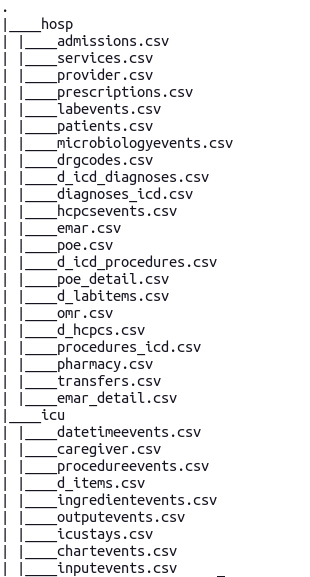
\includegraphics[width=0.5\textwidth]{Figure/MIMIC-IV_tree.png}
    \caption{MIMIC-IV structure}
    \label{fig:mimic-iv-structure}
\end{figure}


\subsection{Hospital data}

Hospital data stores information about patients' admission, basic information, result of laboratory tests, patients' diagnosis, and other general information.
Looking deeper into the hospital data, we can see that it is divided into several tables, each of which stores different types of information.
It is easy to notice that there are some table with "d\_" prefix, which means that these tables store definitions of the data in other tables.

For example, in "d\_icd\_diagnoses" table, we can find information about the International Classification of Diseases (ICD) codes, representing in columns: icd\_code, icd\_version, long\_title.
This table describes respectively the code for the diagnose, the version of the code (currently in MIMIC-IV, both version 9 and 10 are supported) and finally the description of the the diagnosis which is its technical name.
Its code and version are referred in the other table like "diagnoses\_icd" table to mark patients with positive diagnosis of the disease.
Thank to them, I could find the ICD codes for DKA and CKD to identify patients with DKA and exclude patients with CKD.

With "d\_icd\_procedures" table, we can find information about which procedures were performed on patients, representing in columns: icd\_code, icd\_version, long\_title.
It is very helpful to determine the interventions that were performed on patients, which could affect the risk of AKI in DKA patients.

In "d\_labitems" table, we can find information about the laboratory tests that were performed on patients, representing in columns: itemid, label, fluid, category. Column "itemid" is the unique identifier for each laboratory test and will be referred by other tables like "labevents" table to store the result of the test for each patients. Other columns are the label or name of the test, the fluid that was tested (e.g. blood, urine, etc.), and the category of the test (e.g. chemistry, blood gas, etc.).
As laboratory tests contains many important features used in predicting the risk of AKI in DKA patients, this table helps in identify the itemid of the tests that are relevant to the prediction.

Table "d\_hcpcs" stores information about the Healthcare Common Procedure Coding System (HCPCS) codes, representing in columns: hcpcs\_code, short\_description, long\_description.
This table functions similarly to the "d\_icd\_procedures" table, but it uses HCPCS standard which is primarily used in the United States of America.

The remaining tables in the hospital data store information associated with individuals.
Thus, they commonly include "subject\_id" column, which is an unique identifier for each patient and "hadm\_id" column - an unique identifier for each hospital admission.

In "admissions" table, we can find information about patients' admission, representing in columns: subject\_id, hadm\_id, admittime, dischtime, deathtime, admission\_type, admit\_provider\_id, admission\_location, discharge\_location, insurance, language, marital\_status,race,edregtime,edouttime,hospital\_expire\_flag.
Column "admittime" is the time when the patient was admitted to the hospital,
"dischtime" is the time when the patient was discharged from the hospital,
"deathtime" is the time when the patient died (this date were collected 2 years after the last patients recoded got discharged from the hospital),
"admission\_type" is the type of admission (e.g. URGENT, OBSERVATION ADMIT, etc.),
"admit\_provider\_id" is the identifier of the provider who admitted the patient and could be found in "provider" table,
"admission\_location" and "discharge\_location" are the medical facility where the patient was admitted and was discharged,
"insurance" is the type of insurance the patient has,
"language" is the language spoken by the patient,
"marital\_status" is the marital status of the patient.
In this table, I focus mostly on "admittime" and identified columns to match DKA-ICU cases with the corresponding geographical features.

Table "labevents" stores information about the laboratory tests that were performed on patients, representing in columns: labevent\_id, subject\_id, hadm\_id, specimen\_id, itemid, order\_provider\_id, charttime, storetime, value, valuenum, valueuom, ref\_range\_lower, ref\_range\_upper, flag, priority, comments.
Column "labevent\_id" is the unique identifier for each laboratory test, and "itemid" is the reference to "d\_labitems" table.
The time when the test was performed and stored in hospital databases can be found in "charttime" and "storetime".
Both "value" and "valuenum" is the result of the test. It is documented that "value" is the more readable representation of the result while "valuenum" is the numerical value.
The remaining columns are used in medical and monitoring purposes. 

Patients' encoded information are stored in "patients" table, representing in columns: subject\_id, gender, anchor\_age, anchor\_year, anchor\_year\_group, dod.
The anchor\_year is a deidentified year occurring sometime between 2100--2200, and the anchor\_year\_group is a three year long date ranges between 2008--2019. 
These pieces of information allow researchers to infer the approximate year a patient received care.
For instance, if a patient's anchor\_year is 2158, and their anchor\_year\_group is 2011--2013, then any hospitalizations for the patient occurring in the year 2158 actually occurred sometime between 2011--2013. 
Finally, the anchor\_age provides the patient age in the given anchor\_year. 
If the patient was over 89 in the anchor\_year, this anchor\_age has been set to 91 regardless of the actual age of the patient.
To calculate the actual age of the patient, the following formula can be used: 
\begin{equation}
    actual\_age = anchor\_age + anchor\_year - anchor\_year\_group
\end{equation}

Diagnose information are stored in "diagnoses\_icd" table, representing in columns: subject\_id, hadm\_id, seq\_num, icd\_code, icd\_version. 
By referencing table "d\_icd\_diagnoses", we can find the description of the diagnose by the code and version and identify who has DKA and CKD stage 5.


% other unrelated tables 
% services, provider, prescription, microbioevent, drgcodes, hpcpevent, emar, poe, poe_detail, omr, pharmacy, transfer, emar_detail,  

The rest of hospital tables store information for billing and controlling purposes so they are not considered deeply in this thesis. 
For example, table "services" stores information about the services that were provided to patients, representing in columns: subject\_id, hadm\_id, transfertime, prev\_service, curr\_service. 
And "provider" has a single column "provider\_id" which is the unique identifier for each provider.
Table "prescription" provides data related to prescriptions issued to patients, including medication details (name, dosage, frequency), prescribing physician, and date/time of prescription.
Details of microbiology test results, including microorganisms identified, antibiotic sensitivity results, and other relevant microbiological data are stored in "microbioevent".
Table "dgrcodes" or Diagnosis-related group codes contains codes assigned to patients for billing and classification purposes, indicating the type of treatment received.






\subsection{Intensive Care Unit data}

ICU data includes information about patients during their stay in the ICU, including vital signs, medications, interventions, and other information that is recorded promptly.



\section{Tên của nội dung chi tiết thứ 2}


\end{document}